\documentclass[12pt]{article}
%%% ========== Package setup ==========
\usepackage{listings}   % Script listing package
\usepackage{wrapfig}    % Wrap Figure or table package
\usepackage{multicol}   % Multicolumn package
\usepackage{pdfpages}   % Include pdf files

%%% ========== Format setup ==========
%% Setup chinese words encoder
\usepackage{xeCJK}
\XeTeXlinebreaklocale "zh"
\XeTeXlinebreakskip = 0pt plus 1pt

%% More word fonts
\usepackage{fontspec}
\setmainfont{Times New Roman}
\renewcommand{\familydefault}{\rmdefault}
\setCJKmainfont{標楷體}

%% Chinese paragraph format
\usepackage{indentfirst}
\setlength{\parindent}{2em}

%% Page margin
\usepackage[a4paper, total={6in,8in}]{geometry}

%%% ========== Document ==========
\begin{document}

\newcommand{\MakeTitlePage}[1]{
\begin{titlepage}
    \begin{center}

        \fontsize{50}{10}
        \selectfont
        Optimal Control

        \vspace{1cm}

        \fontsize{30}{10}
        \selectfont
        Final exam

        \vspace{11cm}

        \begin{tabular}{ r l }
            班級: & 航太四A \\ [10pt]
            姓名: & 吳柏勳 \\ [10pt]
            學號: & 407430635 \\ [10pt]
            座號: & 3 \\ [10pt]
        \end{tabular}

    \end{center}
\end{titlepage}
}
\MakeTitlePage{6}
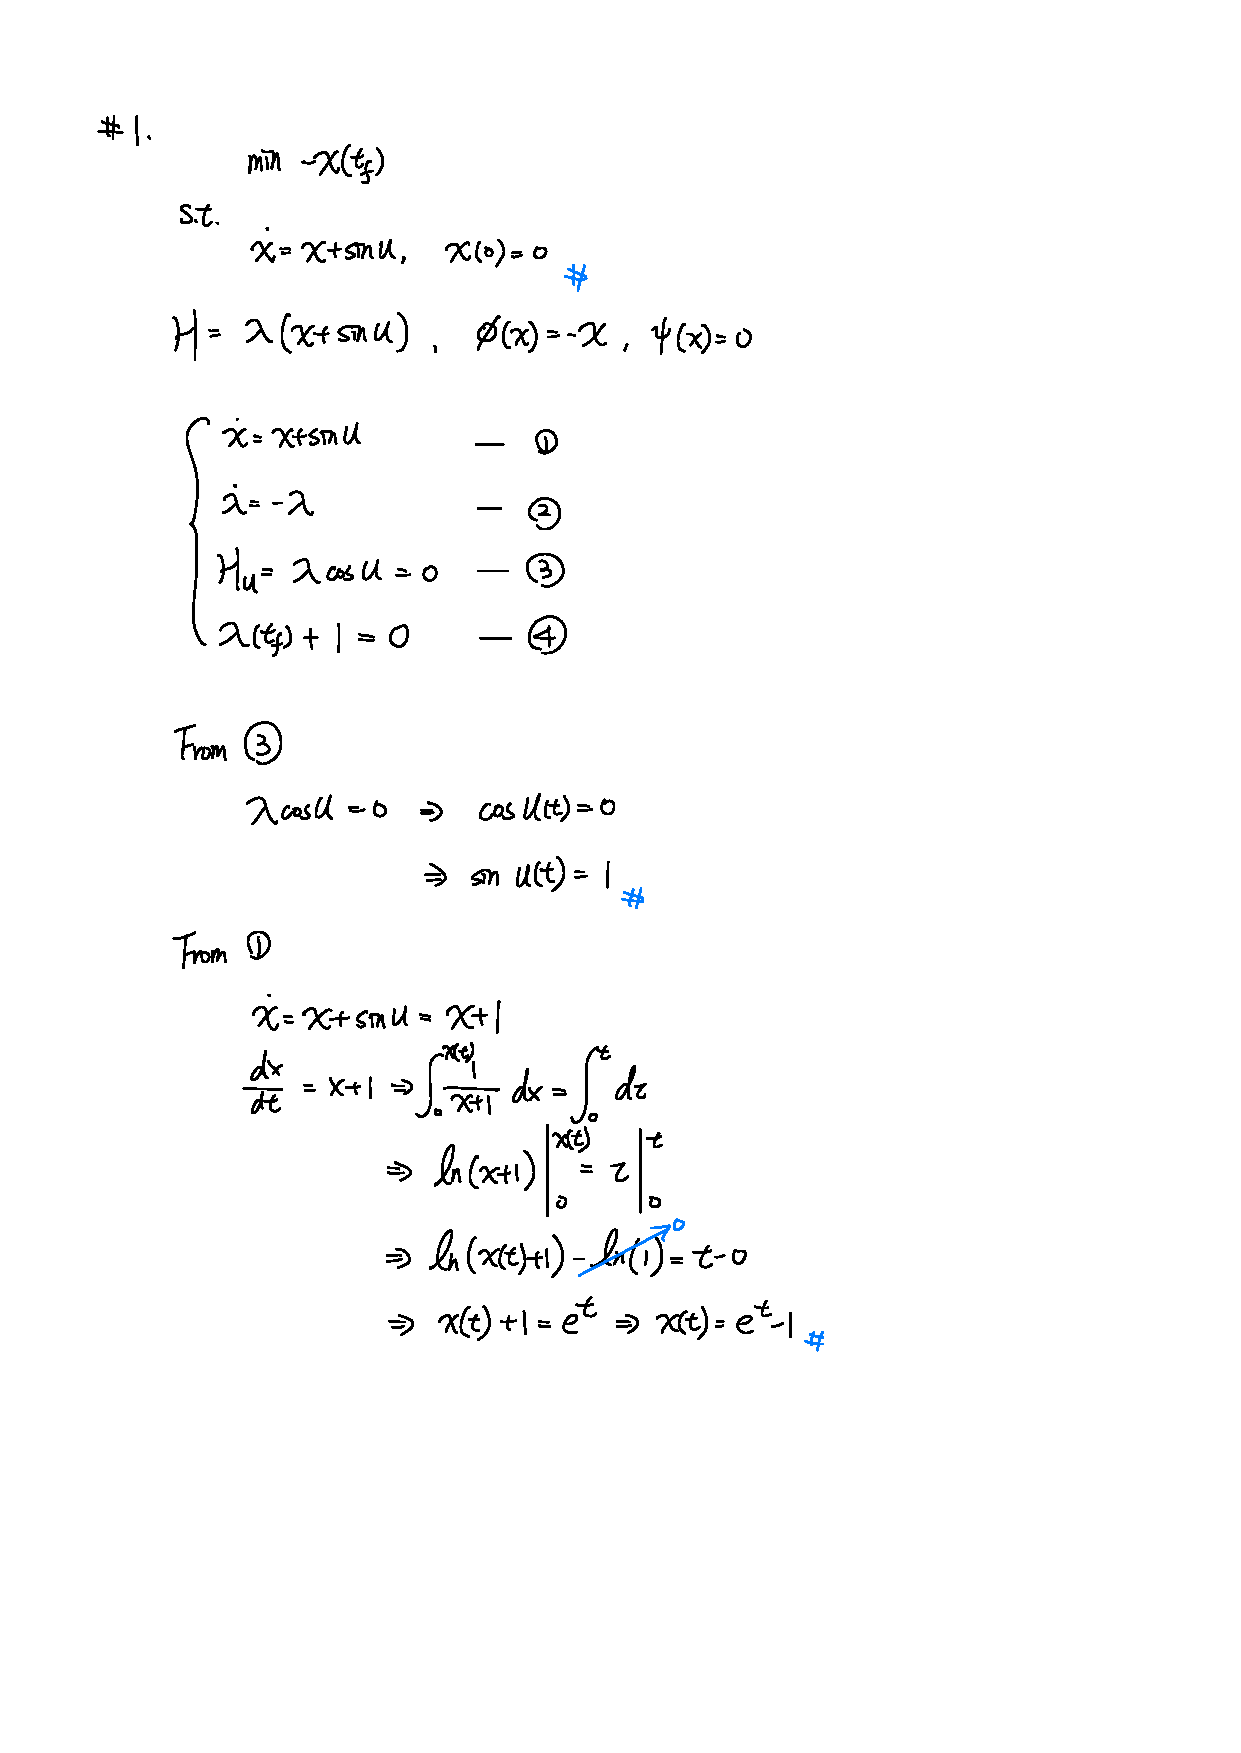
\includepdf[pages=-]{handout.pdf}

% ===================================================================
\subsection*{\#2}

\begin{verbatim}
clear;clc;close All
% Define u(t) is a constant A
init_A = 1;

[A, Jmin] = fminsearch(@fminfunc, init_A);
u = A
Xmax = -Jmin
\end{verbatim}

\begin{verbatim}
function J = fminfunc(A)
    EOM = @(t, x) x+sin(A);
    [~, x] = ode45(EOM, [0 2], 0);
    J = -x(end);

end
\end{verbatim}

        \color{lightgray} \begin{verbatim}
u = 1.5708


Xmax = 6.3891
\end{verbatim} \color{black}


% ===================================================================
\subsection*{\#3}

\begin{verbatim}
clear;clc;close all
init_lambda = 1;
options = optimoptions('fsolve','Display','off');

lambda0 = fsolve(@forwardfunc, init_lambda, options)
[t, state] = ode45(@ODE, [0 2], [0; lambda0]);
Xmax = state(end,1)
\end{verbatim}

\begin{verbatim}
function F = forwardfunc(lambda0)
    [~, state] = ode45(@ODE, [0 2], [0; lambda0]);
    F = state(end,2) - (-1);

end
\end{verbatim}

        \color{lightgray} \begin{verbatim}
lambda0 = -7.3891


Xmax = 6.3891
\end{verbatim} \color{black}


% ===================================================================
\subsection*{\#4}

\begin{verbatim}
clear;clc;close all
init_xf = 7;
options = optimoptions('fsolve','Display','off');

xf = fsolve(@backwardfunc, init_xf, options);
Xmax = xf
\end{verbatim}

\begin{verbatim}
function F = backwardfunc(xf)
    [~, state] = ode45(@ODE, [2 0], [xf; -1]);
    F = state(end,1) - 0;

end
\end{verbatim}

\color{lightgray} \begin{verbatim}
Xmax = 6.3891
\end{verbatim} \color{black}

\subsection*{functiuon for necessary condition}

\begin{verbatim}
function dstate = ODE(~, state)
    % state: [x; lambda]
    u = acos(0);
    dstate = zeros(2,1);
    dstate(1) = state(1)+sin(u);
    dstate(2) = -1*state(2);

end
\end{verbatim}



\end{document}

